\documentclass[aspectratio=169]{beamer}
\usepackage{amsmath, amssymb, amsfonts, amsthm}
\usepackage{cancel}
\usepackage[output-complex-root=j]{siunitx}
\usepackage[american, nooldvoltagedirection]{circuitikz}
\usepackage{bm}
\usepackage{listings}
\usepackage{graphicx}
\usepackage{hyperref}

\usetheme{Berkeley}
\usefonttheme[onlymath]{serif}
\AtBeginSection[]{
    \begin{frame}
    \vfill
    \centering
    \begin{beamercolorbox}[sep=8pt,center,shadow=false,rounded=false]{title}
    \usebeamerfont{title}\insertsectionhead\par
    \end{beamercolorbox}
    \vfill
    \end{frame}
}

\newcommand{\N}{\mathbb{N}}
\newcommand{\Z}{\mathbb{Z}}
\newcommand{\Q}{\mathbb{Q}}
\newcommand{\R}{\mathbb{R}}
\renewcommand{\C}{\mathbb{C}}

\title{EECS 16B CSM}
\author{Bryan Ngo}
\date{2020-10-05}
\institute{Computer Science Mentors}

\begin{document}

\begin{frame}
    \maketitle
\end{frame}

\begin{frame}
    \frametitle{Overview}

    \tableofcontents
\end{frame}

\begin{frame}
    \frametitle{Announcement}

    \begin{itemize}
        \item Google Form later today
    \end{itemize}
\end{frame}

\section{Filters}

\begin{frame}
    \frametitle{Why?}

    \begin{itemize}
        \item allows us to isolate desired frequency ranges
        \item color organ: basically just a visualizer
        \item sort of related to Fourier transform
        \item \href{https://youtu.be/OBM5T5_kgdI}{Afrotechmods video}
    \end{itemize}
\end{frame}

\begin{frame}
    \frametitle{Types}

    \begin{itemize}
        \item low-pass: let in low \(\omega\)
        \item high-pass: let in high \(\omega\)
        \item band-pass: let in range of \(\omega\)
        \item band-stop: block out range of \(\omega\)
    \end{itemize}

\end{frame}

\begin{frame}
    \frametitle{Transfer Functions}
    
    \begin{align}
        H(j \omega) = \frac{V_{out}}{V_{in}} &= \frac{(j \omega)^{N_z}}{(j \omega)^{N_p}} \frac{\alpha_0 + (j \omega) \alpha_1 + \cdots + (j \omega)^n \alpha_n}{\beta_0 + (j \omega) \beta_1 + \cdots + (j \omega)^m \beta_m} \\
        &= K \frac{(j \omega)^{N_z}}{(j \omega)^{N_p}} \frac{\left(1 + j \frac{\omega}{\omega_{z1}}\right) \left(1 + j \frac{\omega}{\omega_{z2}}\right) \cdots \left(1 + j \frac{\omega}{\omega_{zn}}\right)}{\left(1 + j \frac{\omega}{\omega_{p1}}\right) \left(1 + j \frac{\omega}{\omega_{p2}}\right) \cdots \left(1 + j \frac{\omega}{\omega_{pn}}\right)}
    \end{align}
    \begin{itemize}
        \item \(N_z\): number of zeroes
        \item \(N_p\): number of poles
        \item \(\omega_{zn}\): \(n\)-th zero
        \item \(\omega_{pn}\): \(n\)-th pole
    \end{itemize}
\end{frame}

\section{Bode Plots}

\begin{frame}
    \frametitle{Definition}
    \begin{columns}
        \column[]{0.5\textwidth}
        \centering
        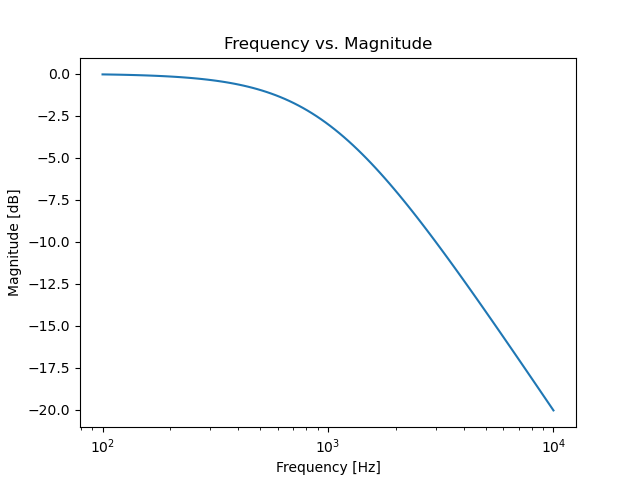
\includegraphics[width=0.8\textwidth]{Figure_1.png}

        \column[]{0.5\textwidth}
        \centering
        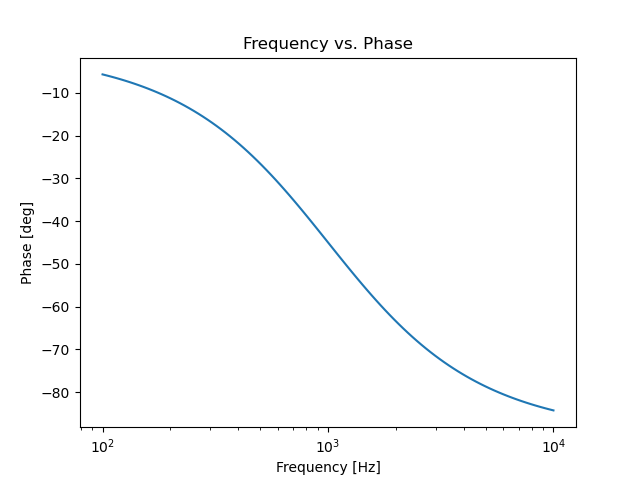
\includegraphics[width=0.8\textwidth]{Figure_2.png}
    \end{columns}
    \begin{itemize}
        \item comes in pairs: magnitude \& phase
        \item above: low-pass filter
    \end{itemize}
\end{frame}

\begin{frame}
    \frametitle{Features}

    \begin{itemize}
        \item magnitude
        \begin{itemize}
            \item \(x\)-axis: log frequency (\si{\hertz})
            \item \(y\)-axis: \(|H(j \omega)|\) (\si{\deci\bel} or intensity)
            \item \textbf{cutoff frequency}: \(|H(j \omega)| = \frac{1}{\sqrt{2}} = \SI{-3}{\deci\bel}\)
        \end{itemize}
        \item phase
        \begin{itemize}
            \item \(x\)-axis: log frequency (\si{\hertz})
            \item \(y\)-axis: phase offset (\si{\degree} or \si{\radian})
        \end{itemize}
    \end{itemize}
\end{frame}

\begin{frame}
    \frametitle{Why?}

    \begin{itemize}
        \item allows us to characterize a filter very fast
        \item quick visual tool
    \end{itemize}
\end{frame}

\end{document}
